\documentclass{template}
\usepackage{color}
\usepackage[hyphens]{url}
\usepackage{longtable}
\usepackage{graphicx}
\usepackage{enumitem}
\usepackage{pdfpages}
\usepackage{hyperref}

\def\etal{{\it et al.~}}
\newenvironment{packed_enum}{
\begin{enumerate}
  \setlength{\itemsep}{1pt}
  \setlength{\parskip}{0pt}
  \setlength{\parsep}{0pt}
}{\end{enumerate}}
\newenvironment{packed_item}{
\begin{itemize}
  \setlength{\itemsep}{1pt}
  \setlength{\parskip}{0pt}
  \setlength{\parsep}{0pt}
}{\end{itemize}}

\begin{document}

\title{Tor's Usability for Censorship Circumvention}
\numberofauthors{1}
\author{
 \alignauthor Linda N. Lee, David Fifield, Nathan Malkin \\
   \vspace{0.5em}
   \affaddr{University of California, Berkeley} \\
   \affaddr{\{lnl,fifield,nmalkin\}@cs.berkeley.edu}\\
}
\maketitle

\begin{abstract}
Tor has grown beyond its original purpose as an anonymity tool and has 
since become an important censorship circumvention tool. It is now listed
as one of the ways that normal people use Tor \cite{whotor}.
We specifically examine its usability as a censorship circumvention tool,
an essential facet for adoption and use.  
We focus our analysis on the connection configuration interface of Tor browser,
as censorship circumvention requires correct transport configurations.
We will conduct a large-scale user study examining 60-100 of users 
on how they navigate Tor's configuration wizard to complete seven browsing tasks 
in three different adversarial settings. Our study combines quantitative measurements (interface
paths taken to success, time to success, and which configuration was chosen) and
qualitative measurements (if users were comfortable with use, what was most confusing, and 
if they would use the browser again). The first phase of the study will evaluate if and how 
easily users can circumvent censorship using Tor Browser. The second phase
of the study will test improvements to the interface and an alternate interface. 
Our goal is to integrate positive usability changes into the Tor Browser. Since
the configuration interface is modular and does not require changes to the Tor Browser
functionality, these changes will be easy to deploy. 

\end{abstract}

\keywords{Censorship, Security, User Studies, Anonymity, Tor}

\section{Tor}
\noindent {\bfseries Usability}
Tor is primarily known as the most widely used anonymity tool today. 
For this reason, user studies on Tor have been solely about the usability of Tor as an
anonymity tool. Norcie~\cite{norcie2012eliminating} conducted an experiment which identified 
``stopping points'' in Tor browser,  documenting points when people would get frustrated enough 
to stop using Tor. To our knowledge, that has been the only published user study of Tor. 
Since then, Tor has had a lot of updates. There have been been no published usability evaluations of
Tor Browser since the introduction of the 4.0 series, which introduced radical UI changes. 
Lee and Fifield \cite {uxsprint} ran a small pilot study testing the download, install, and user interface of Tor Browser. 
This study uncovered a number of bugs and stopping points. Changes made are reflected in series 
5.1 and later. \\

\noindent {\bfseries Scoping}
There are still many features of Tor that are left unevaluated through user
research --- such as advanced web tasks (e.g., accessing hidden services), the
configuration menu to connect to the Tor network, configuring automatic
updates, and identity/cookie management. Rather than selecting the features to
study in isolation,
we decided to focus on an important use case of Tor browser: censorship circumvention. 
Internet censorship is pervasive across the world today \cite{faris2008measuring}, with 
some countries blocking censorship circumvention tools as well \cite{winter2012great}. 
To our knowledge, this is the first user study investigating the usability of Tor as a 
censorship circumvention tool.\\

\noindent {\bfseries Motivation}
Changing the configuration interface would not require changes to the 
Tor Browser functionality, making any suggested improvements very practical to 
deploy in a short period of time. {\color {red} Additionally, people are just literally
being censored everywhere so a lot of people are using it for this purpose. So 
we want this to be usable for that purpose.} 

\section{The Configuration Interface}

\noindent {\bfseries Overview}
The Tor Browser provides a configuration interface to guide users through setting up 
their connection to the
Tor network. While people in most countries can connect to Tor using the
dialog's default settings, citizens in certain censorship environments must
make use of additional settings, such as bridges, proxies, or both. 
(Bridges are unlisted Tor relays, with pluggable transports to obfuscate traffic.
Proxies help bypass local network restrictions and are typically only
needed in restricted cases such as corporate environments.)
Our study explores how successfully this interface guides users to
correctly configuring their browser.\\

\noindent {\bfseries Configuration Flow}

\begin{figure*}[t]
\label{fig:interface}
  \centering
    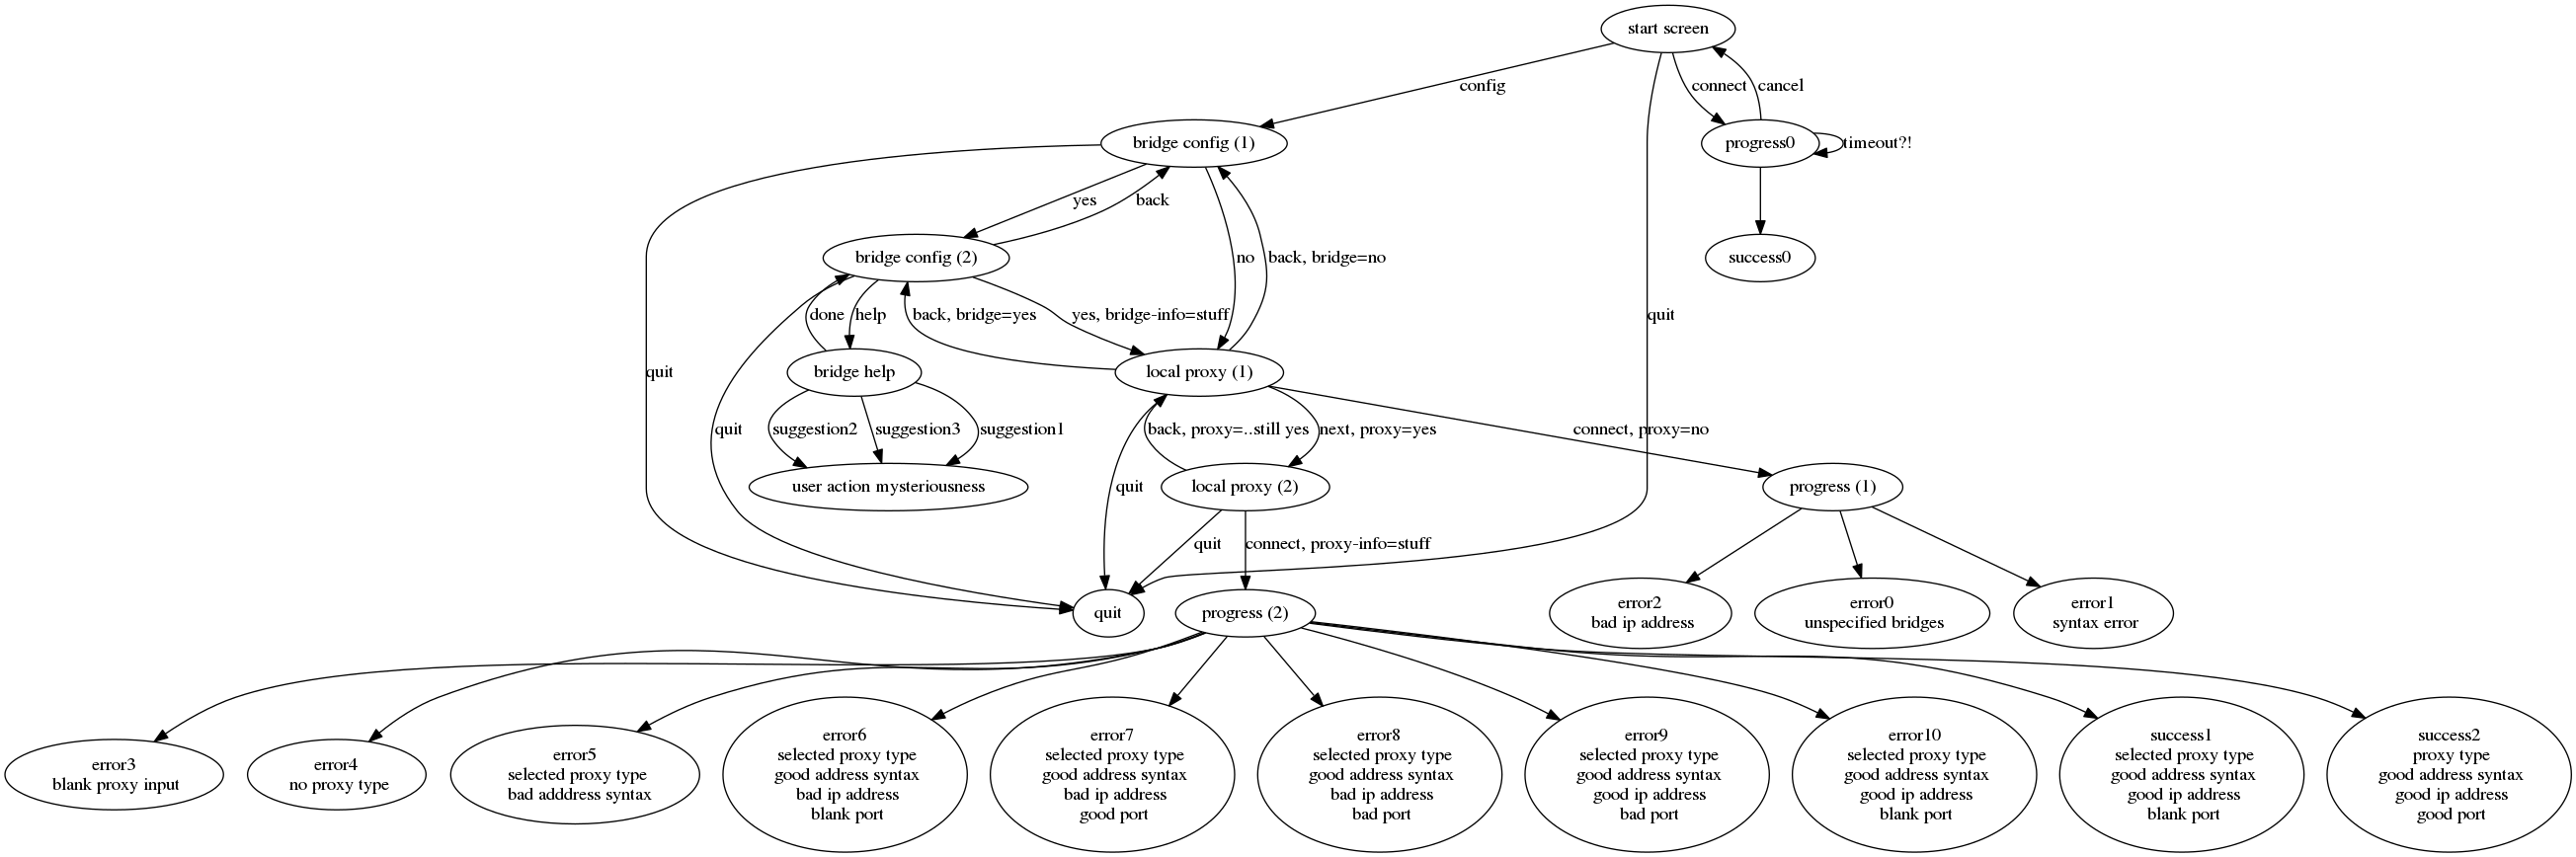
\includegraphics[width=\textwidth]{../torconfig.png}
    \caption{This flow chart shows all of the possible paths taken through the
    Tor configuration interface. A state represents a window in the interface,
    with the exception of the leaves, which indicate the final action taken by
    the interface (``q'' for quit, ``s'' for success, and ``e'' for error). The
    transitions between the states indicate which user action causes that
    transition. Annotations for the error states can be found by following
\href{https://github.com/lindanlee/circumvention-ux-tor/blob/master/torconfig.dot}{this hyperlink}.}
\end{figure*}

As bridges and proxies can be configured independently or together, there are
four main ways to set up a connection:

\begin{enumerate} \itemsep1pt \parskip0pt \parsep0pt
    \item With a bridge and proxy
    \item With a bridge but no proxy
    \item Without a bridge but with a proxy
    \item Without either a bridge or proxy
\end{enumerate}

The launcher interface asks a series of questions to
determine which of these configuration states a user requires.
The four high-level states correspond to five distinct paths through the
configuration interface. (The latter option -- connecting with neither a bridge
nor proxy -- contributes two separate paths.) Each path branches further
depending on user-specific inputs. Figure \ref{fig:interface} illustrates the
resulting paths. 

When the configuration window opens, a user is given the option to connect
directly to the Tor network by clicking ``Connect'', or to click ``Configure''
``if this computer's Internet connection is censored or proxied'' (Figure
\ref{fig:window1}).

If they choose the latter, the next screen asks, ``Does your Internet Service
Provider (ISP) block or otherwise censor connection to the Tor network?''
(Figure \ref{fig:window2}). Though this sounds repetitive, it is meant to
identify and divert users who need only a proxy (and no bridge).
This phrasing of the question carries the assumption that people will
not know if they need a bridge or not, but that they are equipped to answer if their
current network environment censors the Tor Network. 

\begin{figure}[h]
\label{fig:bridges}
  \centering
    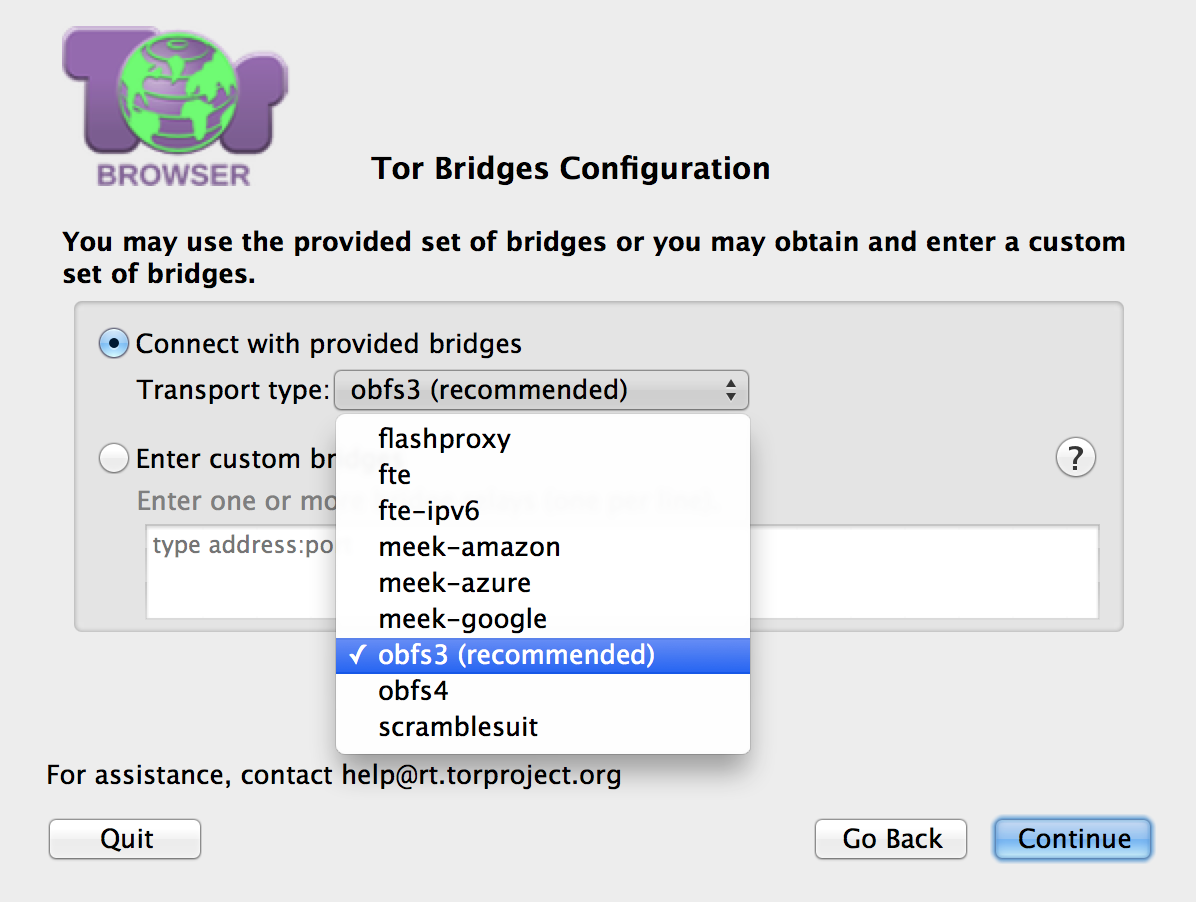
\includegraphics[width=0.5\textwidth]{configuration-screenshot.png}
    \caption{The Tor Bridges Configuration window of the Tor configuration
    interface. Tor users in censored environments and some of our participants
    will be required to select the correct bridge for circumventing censorship.
    Note that the interface prompts users to choose a transport type, which can be
    the source of confusion. Bridges are non-listed guard relays to the Tor
    network; transports, supported by bridges, obfuscate traffic in
    different ways.}
\end{figure}

Next, users are asked to configure bridges by selecting a transport type from a
dropdown menu or entering the IP address of a custom bridge in a textbox (Figure
\ref{fig:bridges}).
Finally, users are asked whether they need a local proxy (Figure
\ref{fig:window4}) and (if they answered yes) to configure it (Figure
\ref{fig:window5}).

Note that a user can decide to click ``Configure'' on the first screen, but then
opt out of both bridges and proxies.
In this case, connecting after these configuration steps
would be equivalent to clicking ``Connect'' on the first screen. \\ 

\noindent {\bfseries Design choices}
The launcher interface utilizes a number of techniques to aid users and simplify
the choices they have to make. Help buttons and a support email address that
appears on every screen are meant to assist users that get stuck in the process.
The interface also makes good use of defaults, for example by emphasizing that
certain options ``will work in most situations.''

Still, there remains potential for confusion, especially with the more advanced
configuration options. Bridges and proxies are not clearly defined, the
interface doesn't specify when they would need to be used, and there is limited
guidance for how to correctly choose specific values (e.g., which transport type
to use or where to find proxy settings).

\section{Hypotheses}
We expect that the average user will
struggle to connect because they lack knowledge of the technical terms and
mechanisms required for circumvention (such as pluggable transports) and cannot
obtain information not explicitly provided by the user interface (e.g., IP
addresses of non-publicly listed bridges).

\begin{itemize} \itemsep1pt \parskip0pt \parsep0pt
\item  {\bfseries H1}: people don't know what a bridge or proxy is. > ask participants to define these terms in the survey.  
\item  {\bfseries H2}: people don't know what the difference between a bridge and a proxy is > ask if people can distinguish them. 
\item  {\bfseries H3}: people do not know when bridges or proxies are necessary > ask them this in the survey.  
\item  {\bfseries H4}: proxies cause confusion when configuring bridges. screen recording: see if people click on proxies (none of the environments require a proxy)
\item  {\bfseries H5}: people will favor familiar-sounding transports (i.e. meek-google versus meek-azure or scramblesuit) > see screen recordings, ask in survey for which transports were picked in which order and why they chose the final transport.  
\item {\bfseries H6}: (some dialogue is redundant. see opening window: "before you connect..." and bridge2 window: "you may use...") > we can try asking if people find these things useful, if they would prefer the interface without it, or if they read it.  
\end{itemize} 

\section{Methodology}

To test our hypotheses, we simulated several environments in which people may
have to use Tor for censorship circumvention. We examined whether users are able
to join the network and studied how they interact with the launcher interface.
Based on our findings, we designed improvements to the Tor launcher interface,
which we test in a large-scale study.

\subsection{Simulated censorship environments}
We simulated three censorship environments.
They are informed by our experience with pluggable transports
and knowledge of commonly seen censorship techniques.
They are not meant to perfectly replicate the network environment
in any particular country. Although inspired by reality, these
abstract simulations are intended to require distinct configurations
of the Tor Browser from our participants.

\begin{itemize} \itemsep1pt \parskip0pt \parsep0pt
\item {\bfseries Mild censorship} 
(Representative of countries such as France and Australia.)
Certain domains are blocked. Reaching these 
domains requires a censorship circumvention 
tool. The default option to ``connect'' to the Tor network 
directly will circumvent this censor. Additional correct
bridge or proxy configurations are optional. 

\item {\bfseries Intermediate censorship} 
(Representative of countries such as Tunsia.)
Certain domains are blocked. Censorship circumvention
tools such as Tor are blocked. Since all public Tor
relay nodes are blocked, the default option to ``connect'' to the Tor network
directly will fail. Any choice of a hard-coded bridge
or a valid non-public bridge will circumvent this censor.  
Additional correct proxy configuration is optional.

\item {\bfseries Comprehensive censorship} 
(Representative of countries such as China and Syria.)
Certain domains are blocked. Censorship circumvention tools
are thoroughly blocked. Tor is blocked by blocking all public
Tor relay nodes, and the censor has examined source code to block
all hard-coded bridge relays in the configuration interface. The default option
to ``connect'' to the Tor network directly will fail. Most bridges will fail,
but ``meek-amazon,'' ``meek-azure,'' and ``meek-google'' still work.
% TODO: meek-google doesn't work either, right? Should we remove it?
This is because domain-fronting requires censors to block entire CDNs to also
block this transport (which will cause huge collateral blocking damage), making
it resistant to aggressive censorship environments.
(See ~\cite{fifield2015blocking} for additional details.)\\
\end{itemize}

\subsection{Qualitative interface evaluation}
To identify problems with the existing interface, we conducted a series of
qualitative evaluations with a set of users representative of the general
population.

Using established best practices from the field of user experience research
(\cite{howmanyusers}), we recruited five users for each censorship environment.
We pre-screened our participants to have a good mix of gender, age, technical
background, and familiarity with Tor in each environment, and also overall. \\

%Some references to keep in mind when explaining:
%\href{why 5 users}{http://www.nngroup.com/articles/how-many-test-users/}
%\href{screening}{http://www.userfocus.co.uk/articles/screeners.html}
%\href{summative and usability mixed model}{http://www.usabilitybok.org/summative-usability-testing}

\noindent {\bfseries Procedure}
The experiment begins with the participants being informed that they are in a
simulated censorship
environment, where some --- but not all --- websites are blocked. We
instruct them to visit a non-blocked website and a blocked website on a
``standard'' browser (one that is not used for censorship circumvention, such
as Chrome, Safari, or Firefox) to illustrate the situation.
Participants are told that their
role is that of a regular citizen who is trying to visit blocked websites
for non-critical purposes,
and for whom the chance of risk is minimal. This information is given
to achieve
consistency across participants: behaviors may change if the tasks are
critical or if there were great risks associated with configuration mistakes. 

After explaining the situation and the user's role, we
instruct them to complete a set of
tasks which will require visiting blocked websites. Ultimately, the
participants will need to configure their Tor Browser to circumvent the
simulated censorship environment. These tasks have a three-fold purpose of
providing participants with feedback (if they did not correctly configure their
browser, they cannot reach the website), motivating the participants to
configure the browser correctly, and providing the researchers with an
indicator of successful censorship circumvention.
Participants' screens are recorded to capture how they configure
their browser.

After users complete the browsing tasks (or time runs out), we conduct an
interview, collecting qualitative feedback from
participants about their browsing experience as a whole
and the configuration interface specifically.
We ask questions such as
``What was the most challenging part of connecting?''
and
``What is one change you would recommend?''


\subsection{Interface design and iteration}
After completing the qualitative user studies, we analyzed their results to
identify common themes and problems. Based on these, we then designed
improvements to the Tor launcher interface.

To do this, we used an iterative design process, starting with low-fidelity
(paper and pencil) prototypes and then proceeding to higher-fidelity versions.
At each stage, the prototype was clickable, allowing for more realistic
simulation.

We collected feedback from researchers, professors, and Tor users and developers
through the Tor project's mailing lists. We then iterated on the design by
incorporating the comments and suggestions we received into the next version of
the interface.

\subsection{Quantitative evaluation of improvements}
Once the new design of the user interface is finalized, we will conduct a
large-scale quantitative evaluation, to test whether the improvements had a
measurable effect on people's ability to connect to the Tor network.

The experimental procedure will be nearly identical to the procedure for the
qualitative portion of the study, described above. However, rather than
conducting open-ended interviews at the end of the tasks, participants will be
asked to fill out a brief survey. Furthermore, the interface will be
instrumented to collect metrics and statistics for use in analysis and
hypothesis testing.
Some examples of metrics collected include the time spent on each screen, which
paths the user followed, which interface elements they interacted with, and how
often they did so. These will be analyzed in conjunction with high-level metrics
(was the user able to connect to Tor successfully?).

Participants will be split across several different experimental conditions.
Some will be testing the improved user interface, while those in the control
group will be completing the same tasks using the old, unimproved interface. \\
% NOTE: removed mention of the alternate interface, unless there's something to say about it

\noindent {\bfseries Experiment Logistics} 
We plan to recruit up to 100 users for the purpose of this study,
making it the largest user study of Tor to date.  This study will be conducted at the
Experimental Social Science Laboratory (Xlab)
at the University of California, Berkeley, which consists of 36 laptops,
separated by cubicle walls. We will use individual host firewalls to simulate
censorship environments and will record computer screens to capture 
user activity. The total length of the experiment, including briefing, completing the censorship 
circumvention tasks, exit survey, and debriefing, will be about an hour.
Participants will be compensated \$30 for their time, which covers
minimum wage for an hour and any transportation costs to the lab. 
The IRB protocol to run this user study has been approved (2014-12-6995). 


\section{Results}

The qualitative interface evaluation yielded in hours of observation for a set of 16 pre-selected, diverse participants taking various UI paths in different simulated censorship environments. We then interviewed the participants, getting hundreds of words of feedback from our participants. In this section, we will be talking about the insights gathered from the qualitative interface evaluation, which has shaped the re-design of the interface. All of the results are grounded in participants' experiences and feedback, which are available publicly online. The video screen captures from the experiment can be found \href{https://github.com/lindanlee/circumvention-ux-tor/tree/master/sessions/pre/videos}{here}; a summary of each video can be found \href{https://github.com/lindanlee/circumvention-ux-tor/blob/master/sessions/pre/participant-summaries.txt}{here}. The corresponding notes from the after-experiment interview can be found \href{https://github.com/lindanlee/circumvention-ux-tor/tree/master/sessions/pre/notes}{here}. 

We have evaluated at least one Tor user, one participant who has heard of Tor before the study, and three people who had never heard of Tor before in each simulated censorship environment. The nature of small-scale qualitative studies yields in rich information about each participant, but making generalizations from these results such as ``Tor users were able to configure quicker'' would be unsound. Our observations from our particular three participants were that they were more capable of debugging after failure modes and were more methodological about doing so, but they faced similar difficulties as the other participants. 

We noticed four common challenges that our participants have had with the interface:  

\begin{itemize} \itemsep1pt \parskip0pt \parsep0pt
\item {\bfseries Challenge1:} People don't know how to choose between ``connect directly'' versus ``configure'' on the first screen. As seen in Figure \ref{fig:window1}, there is some guidance for the users, but we found this largely unhelpful since people do not understand the text on the screen. 
\item {\bfseries Challenge 2:} People feel compelled to set up a bridge, even if they don't need one, because they do not know how censorship works. Participants knew that they were censored to some degree since we had simulated censorship of websites. However, bridges are only necessary when the government has taken active steps to censor Tor itself.
\item {\bfseries Challenge 3:} When their first attempt to connect fails, people tend to first try changing the proxy settings, because the interface directs people to the last window participants saw before the connection failure. This was problematic since the problem is not necessarily where the interface directs users. For instance, it was common for the interface to redirect users to the proxy window in Figure \ref{fig:window5}, even when they needed to pick another bridge. 
\item {\bfseries Challenge 4:} When the first attempt to connect fails, people did not know what to do or what to try next. The feedback given to users was not understood (see Figure \ref{fig:error}) and also did not guide users into specific actions (such as trying a different bridge, trying the same configuration again, try connecting directly, etc.).
\end{itemize}

\begin{figure}[t]
\label{fig:error}
  \centering
    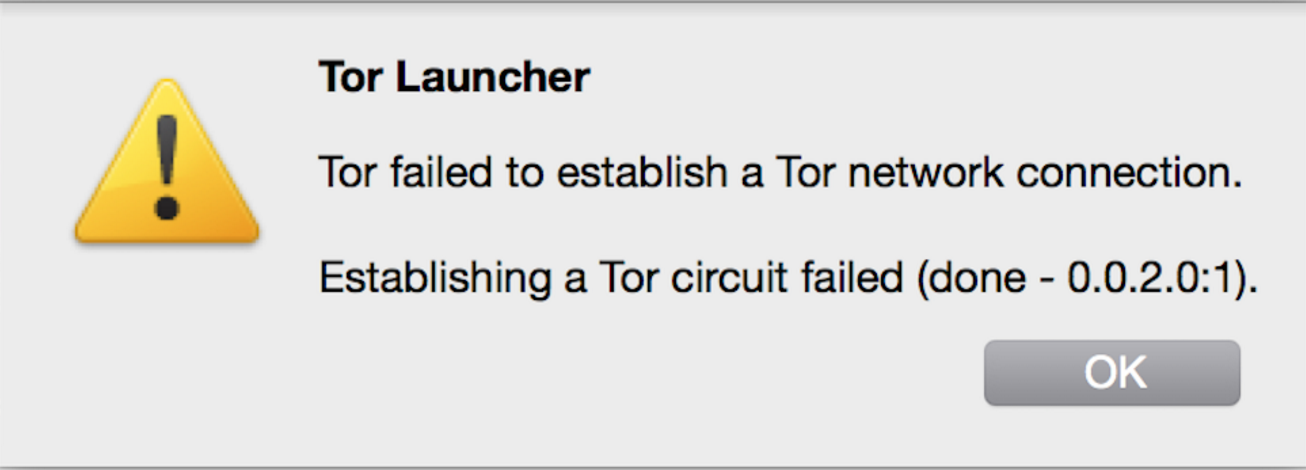
\includegraphics[width=0.5\textwidth]{error.png}
    \caption{An example of a technical error message which our participants did not understand.}
\end{figure}

These common four problems were illustrated by our participants concretely:

\begin{itemize} \itemsep1pt \parskip0pt \parsep0pt
\item {\bfseries Proof of Challenge 1:} Of the five participants who could click directly to the network, three participants (P3,P4,P10) did not choose to connect directly.  Of the eleven participants who needed to configure their connection, eight (P1, P5, P6, P7, P8, P11, P13, P14, P16) chose to connect directly. One participant (P12) clicks configure, but answers the questions in such a way that it creates a direct connection. Only one (P15) was chose to configure when they needed to.
\item {\bfseries Proof of Challenge 2:} Five participants were placed in a censored environment which did not block Tor. Three of the five (P3, P4, P10) configured a bridge for their connection. Of the other two, one participant (P2) was convinced that configuring a bridge was the correct course of action, but was intimidated at the thought of doing so and was pleasantly surprised when a direct connection succeeded; only one participant (P9) believed that a direct connection would work. 
\item {\bfseries Proof of Challenge 3:} All three of our participants (P14, P15, P16) who never were able to circumvent the simulated censorship environment spent 25-30 minutes trying to correctly configure a proxy, which was never necessary to connect to the Tor network. Out of the five participants who needed to fix their bridge settings, there were only two participants (P5, P6) who eventually were able to figure out that their bridge settings needed to be adjusted.
\item {\bfseries Proof of Challenge 4:} One participant (P14) tried the same configuration seven times, even though those settings failed each time. Another participant (P12) tries the same configuration three times, and only manages to connect through a technical artifact of the experiment even though that should not have worked. Both of these participants emphasized that they did not know what they should be doing. Other participants' interview responses also indicate a lack of feedback after failure cases (P8, P15, P16). 
\end{itemize}

The above challenges stemmed from these observations: 

\begin{itemize} \itemsep1pt \parskip0pt \parsep0pt
\item {\bfseries Observation 1: Users lack a mental model of how censorship works.} For instance, our participants did not know the difference between a bridge and a proxy or a censored website versus censored Tor relays. We suspect that this is the result of an accurate mental model of how the Internet works.  It would be unreasonable to assume that users should know this information, but some of this may be required to make a correct decision in the current interface. 
\item {\bfseries Observation 2: The interface flow does not guide users down the ideal path.} Much of the real estate on bridge configuration is used for the ``custom bridges'' option, which is an option rarely used. The interface instructs users to check out Internet settings to see if they would require a proxy, but it turns out that people are not skilled at doing so. Because the interface redirects users to the proxy screen after failing to make a connection, most of our participants tried configuring a proxy after a connection had failed due to an assumption that the proxy was the reason for the failure. In reality, there was no proxy setup required for any simulated censorship environment in our experiment and participants should have configured a bridge. 
\item {\bfseries Observation 3: There is little constructive feedback during failure cases.} When a connection seems to not work, our participants were unsure of if they should wait more or if they should try the connection with the same configuration again, both of which are viable strategies, depending on the situation. Although there are certain error messages which were helpful, most of the error messages were technical and not understood by our participants (Figure \ref{fig:error}). The interface does not give clear directions on what participants should do next if a connection fails. 
\end{itemize}

Although we cannot comment on if the challenges mentioned above will be exactly representative of the Tor user population, it is fair to claim that these challenges are challenges that some Tor users will encounter while configuring Tor. Our observations are grounded in user interaction--specifically user mental modes, UI flow, and failure design--giving us high confidence that addressing these observations will make a noticeable impact on the usability of the Tor configuration dialog for censorship circumvention. 

\section{Design}
Based on the feedback and the insights from our qualitative interface evaluation,
 we designed improvements to the launcher interface. This section
discusses design considerations we employed and corresponding justifications. \\

\noindent {\bfseries Automation}
One common piece of feedback from experts and novices alike was that the
connection process could be simplified with automation. At first glance, many
decisions currently made by the user could be automated. For example, bridge
selection needs to happen only if a regular connection failed, and bridges could
be tried automatically until one succeeds. However, there are security
considerations that make this solution problematic. If the launcher starts by
trying to make unobscured connections to publicly listed relays, detection is
trivial in a country that logs Internet traffic, potentially resulting in
repercussions for citizens. Furthermore, users may be turned off by the
lack of transparency in the connection process.

However, other elements of the process can be automated without adverse effects.
For example, local proxy settings can be imported from other browsers on the
machine by looking for settings in well-known locations on the filesystem. Automatically
detecting the need for a proxy and importing the proxy settings required would save
our participants from a task they do not have the background to easily complete. 
Since this piece of automation offers a significant increase in usability for our users
(addressing our most common failure case) with no apparent risks, we have incorporated it
into our design. \\

\noindent {\bfseries Building a better mental model}
Participants' lack of a mental model of censorship led them to believe their
Tor connection was censored when, in reality, it was not. It furthermore contributed
to their confusion between bridges and proxies. Our design directly addresses
these issues.

Potentially ambiguous text (i.e., referring to censorship) is removed in favor
of stating the underlying options, as it was shown to confuse our participants.
Previously, separate screens with binary options (Do you need a proxy? Yes/No) 
were provided to help users decide if they needed a bridge or proxy, and skipping
the configuration windows for bridges and proxies, respectively, when users
answered that they didn't need one. We have removed these screens
because our participants did not understand how to answer them correctly. This is 
anticipated in the old interface, in fact: written text in the interface guides users on to 
how to answer those questions.  

We chose to display all information about bridges and proxies is now contained on one 
respective screen in the interface, giving the user has the full context of their decision.
We made the guidance from the last interface (to not choose a bridge, to not choose a proxy)
more direct by selecting the  option to opt out of a proxy as the default option on those screens. 
This results in a more streamlined interface with fewer windows
and fewer clicks required for our participants. \\

\noindent {\bfseries Clarifying paths through the interface}
Many users struggled because the workflow implicitly suggested by the interface
didn't match the ideal path: crucial steps to follow were unclear or obscured,
while undue prominence was given to comparatively less important elements.
Our new design inverts this trend, focusing attention on the interface elements
that are more important, or more generally applicable.

A clear example of this is the ``Connect'' button on the first screen, which has
increased in size and become green, making it more prominent as the recommended
option. We believe that this will help the majority of Tor users. 
Although some of our participants in environments had chosen to connect
directly when they needed to configure, this is generally seen as low-risk today, and 
the majority of censorship today can be circumvented with a direct connection. 
A similar aesthetic applies to the connect button seen after custom
configuration.

To help lessen the cognitive load and distribute a representative amount of space
for options, recommendations are selected as the default option, and rarely used 
elements are deemphasized. To encourage our users to click on helpful options, 
the help button on the bridge configuration screen
has been emphasized to be bigger, since it is a helpful option which people rarely
clicked. To discourage our users from using an advanced setting only technical users 
have a chance of  configuring correctly and should only be used in very rare circumstances, 
we have now incorporated the custom bridge configuration in the dropdown menu; 
it previously took up a significant portion of the bridge configuration screen. 

A progress indicator at the top of the window indicates which configuration step
the user is on. It serves to clarify the independence of bridges and proxies,
which need to be configured separately. In the event of a failure, the user is
returned to the first step of the process -- the bridge configuration -- to
avoid misleading users into thinking the proxy settings are the culprit. Previously,
the user had to manually click to go backward in the dialog to configure bridges.
Even in the rare event that the proxy is the issue for the connection setting, the user
will be directed to the proxy page naturally through the flow of the UI, without
having the user to defy the natural flow of configuration. \\

\noindent {\bfseries Designing for failure cases}

Many users were led astray by interface elements that were unhelpful or
misleading if the program encountered connection problems. Our design seeks to
prevent such confusion by anticipating failures and providing specific instructions
for our participants on their next steps.

The progress bar in the connection window drew many complaints, because it got
stuck and didn't offer any guidance for how long users were supposed to wait. 
The connection process can take a non-trivial couple of minutes, and users may
think that the connection isn't working, even when it is making slow progress. We
address this by providing a countdown timer, indicating that a long wait time does
not indicate failure. We further encourage waiting by adding visual indicators
for major milestones in the connection, providing better feedback about what has
been accomplished so far. Additionally, the current status of the connection
attempt (drawn from the log) is displayed, to aid in understanding and
debugging.

In the event that the connection attempt fails, messages from the log are
displayed, along with tips and suggestions about what to do next (e.g., try
another bridge). To make potential the options clearer, the new failure screen
includes a separate button for common next steps which are able to resolve
a failed connection, which are to retry without changing settings and to reconfigure 
the connection. \\

\noindent {\bfseries Additional changes}
In addition to the changes above, we have simplified flows where possible,
provided clearer definitions of bridges and proxies, and reduced visual clutter.
We believe that all of these changes are cohesive with the other design changes
made to the interface and will be beneficial for the user.

\section{Future Work}

We plan to finish the user study by the end of the semester. 
From this experiment, we hope to accomplish the following: 

\begin{itemize} \itemsep1pt \parskip0pt \parsep0pt 
\item {\bfseries Test an improved configuration interface} With the measurements collected
from testing the interface as-is, we will design and test improvements to minimize
time taken, paths taken, and error states reached.
\item {\bfseries Push changes} We have the support of Tor developers
to improve this interface. Additionally, since the configuration interface does not require 
any changes to the Tor Browser functionality, improvements to the interface will
be easy to deploy. 
\end{itemize}

\section{Resources}
\noindent Our online artifacts of the work done during this class, Fall 2015,
are below: 
\begin{itemize} \itemsep1pt \parskip0pt \parsep0pt
\item \href{https://github.com/lindanlee/circumvention-ux-tor}{github repo with experiment plans, code, and paper}
\item \href {https://github.com/lindanlee/circumvention-ux-tor/blob/master/pilot/1-strict.mp4}{pilot video 1}
	\href{https://github.com/lindanlee/circumvention-ux-tor/blob/master/pilot/2-lax.mp4}{pilot video 2}
\item \href{https://github.com/lindanlee/circumvention-ux-tor/blob/master/setup/setup-environment}{experimental setup code: firewall and screen capture} 
\item \href{https://github.com/lindanlee/circumvention-ux-tor/blob/master/setup/takedown-environment}{experimental takedown code: saving files and cleanup} 
\end{itemize}

% from anonymity study
%Our online artifacts of study of Tor as an anonymity tool, such as 
%the summary, results, and resulting browser changes are below:
%\begin{itemize} \itemsep1pt \parskip0pt \parsep0pt
%\item \href{https://trac.torproject.org/projects/tor/wiki/org/meetings/2015UXsprint}{blog post summary}
%\item \href{https://blog.torproject.org/blog/ux-sprint-2015-wrapup}{changes made to Tor}
%\item \href{https://people.torproject.org/~dcf/uxsprint2015/}{subtitled screen videos}
%\end{itemize}

\bibliographystyle{abbrv}
\bibliography{circumvention-experiment.bib} 

\appendix
\section*{A1: Configuration Interface Windows}

\begin{figure}[h]
\label{fig:window1}
  \centering
    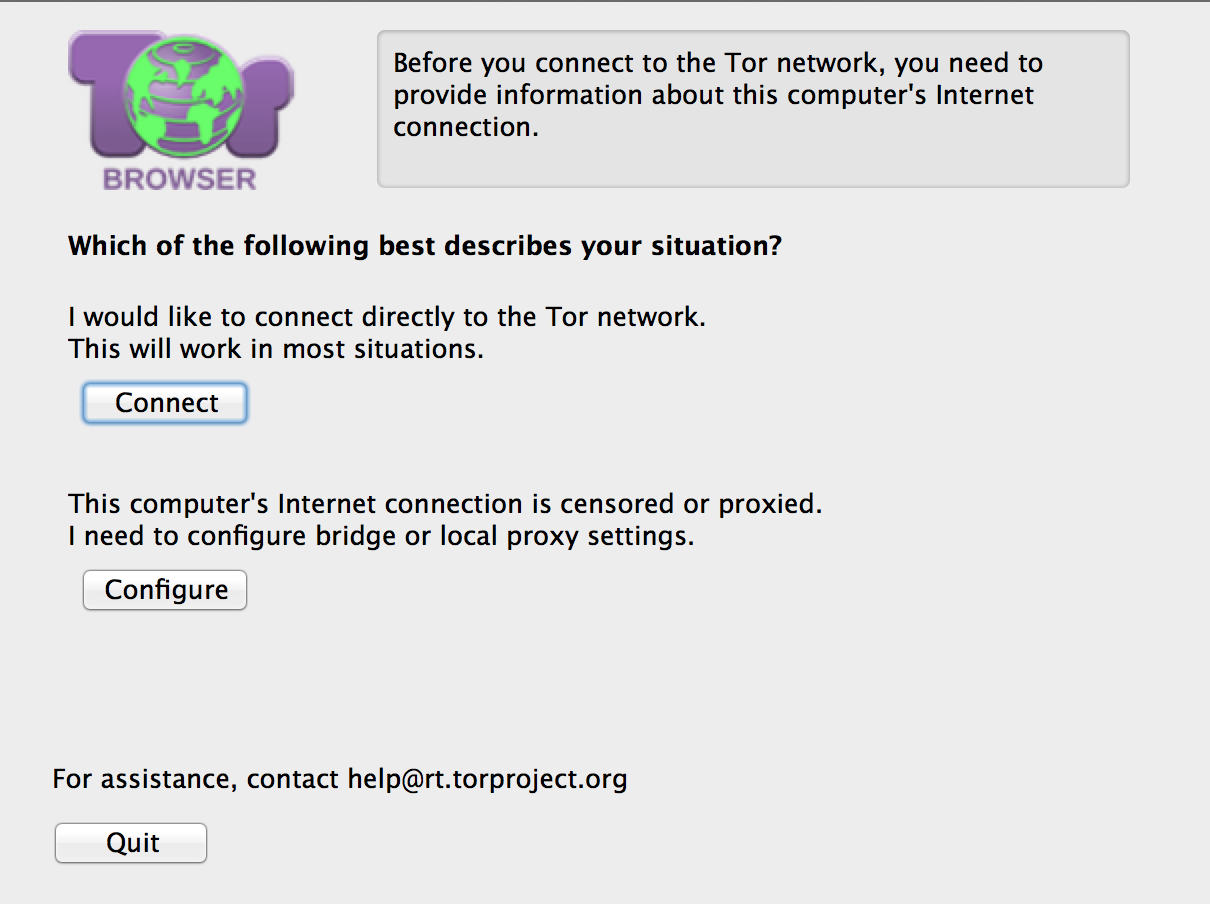
\includegraphics[width=0.5\textwidth]{window1.png}
    \caption{Window 1: the first configuration window shown to the user upon
    starting Tor Browser for the first time. Note that the interface's default choice
    is to connect directly through Tor. The interface also gives additional guidance
    to help users answer this question.}
\end{figure}

\begin{figure}[h]
\label{fig:window2}
  \centering
    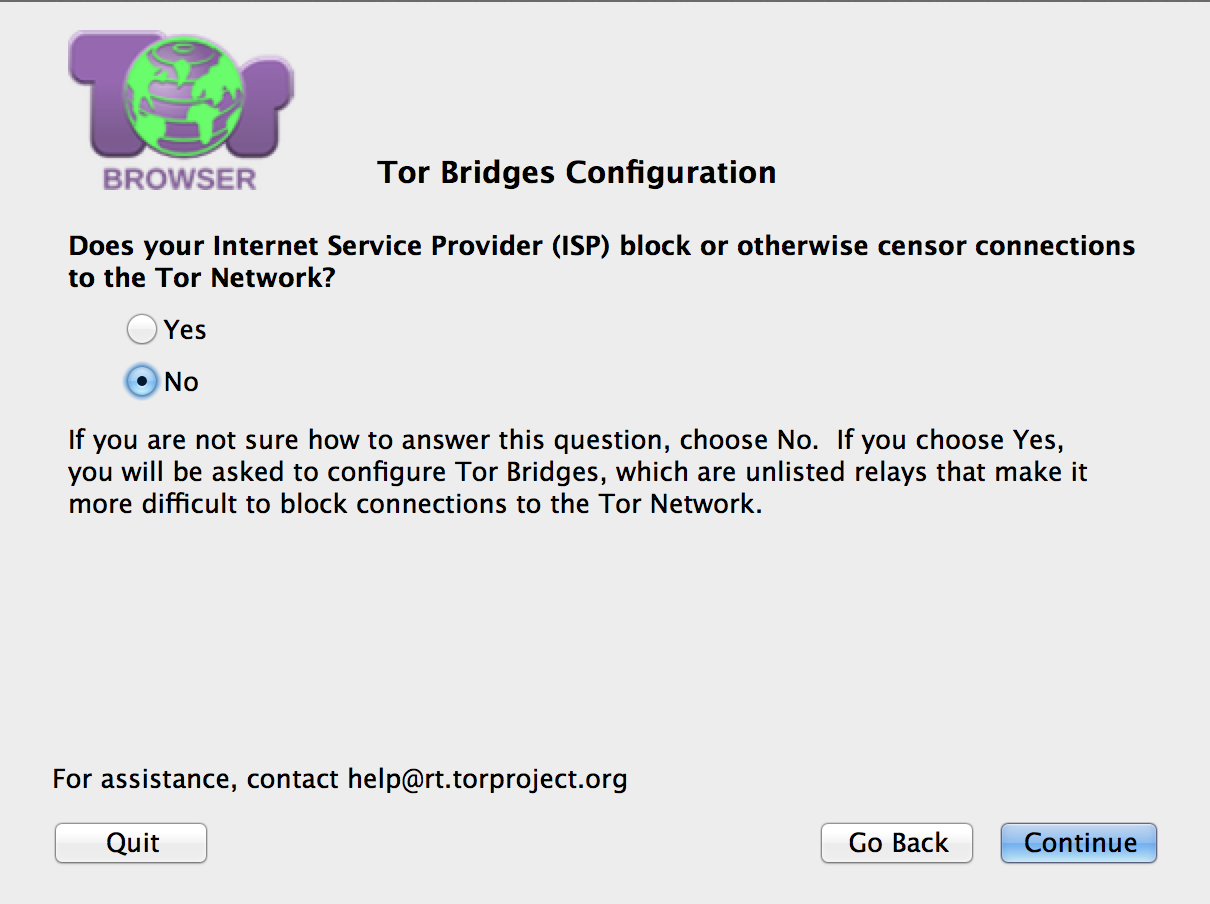
\includegraphics[width=0.5\textwidth]{window2.png}
    \caption{Window 2: This is the next window shown if a user chooses to configure 
    bridges or proxies. Note that the interface's default answer is ``No,'' 
    and also advises users to click ``No'' if they are unsure. The user can navigate to the 
    previous window by clicking ``Go Back,'' and continue configuration by clicking 
    ``Continue.''}
\end{figure}

\begin{figure}[h]
\label{fig:window3}
  \centering
    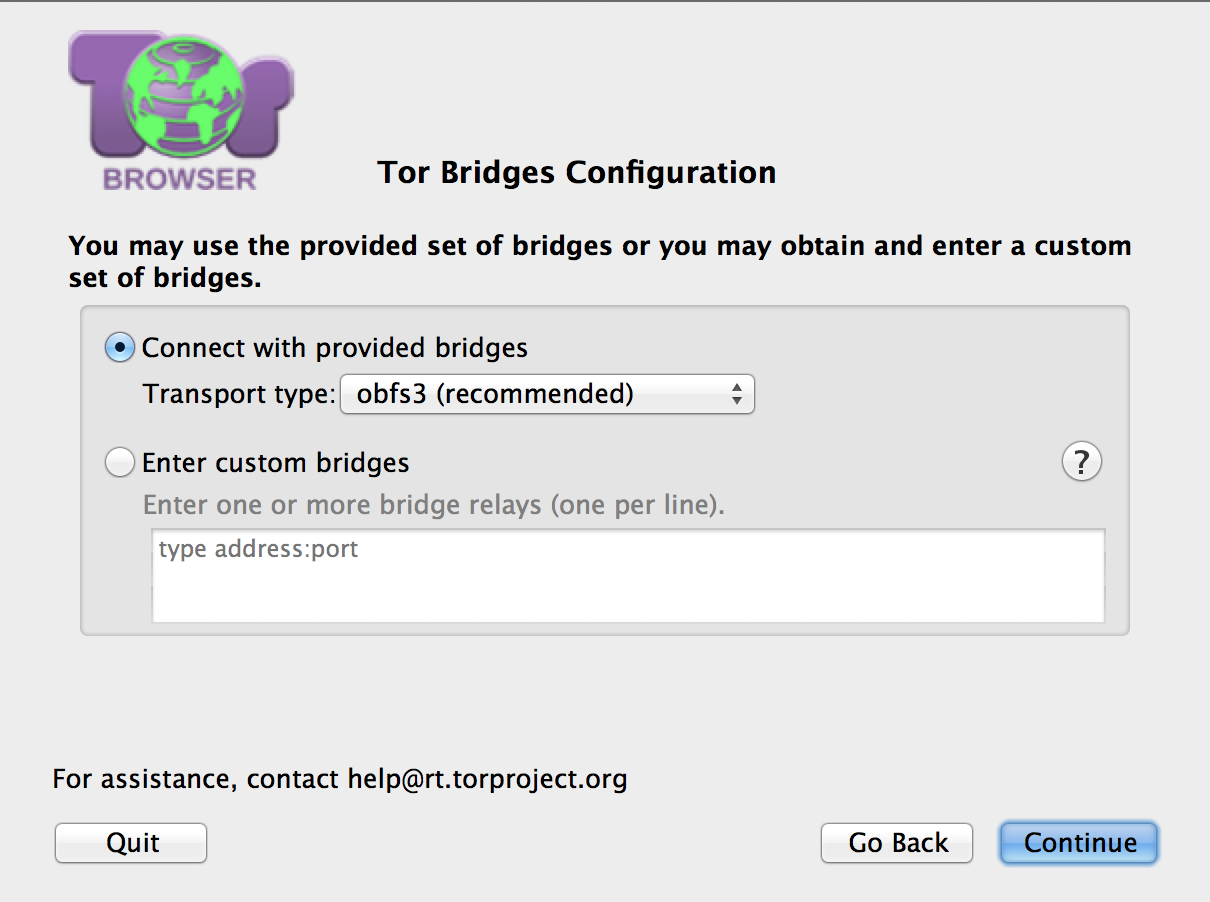
\includegraphics[width=0.5\textwidth]{window3.png}
    \caption{Window 3: This is the window shown when a user answers that a bridge 
    is required for the connection. Note that the default answer is to connect with a hard-
    coded bridge rather than to enter in a custom bridge, and to use the recommended 
    transport (obfs3). A possible source of confusion is that that the user is asked to choose 
    a transport type, when the interface clearly is asking for bridge configuration. The user 
    can navigate to the previous window by clicking ``Go Back,'' and continue configuration 
    by clicking  ``Continue.''}
\end{figure}

\begin{figure}[h]
\label{fig:window4}
  \centering
    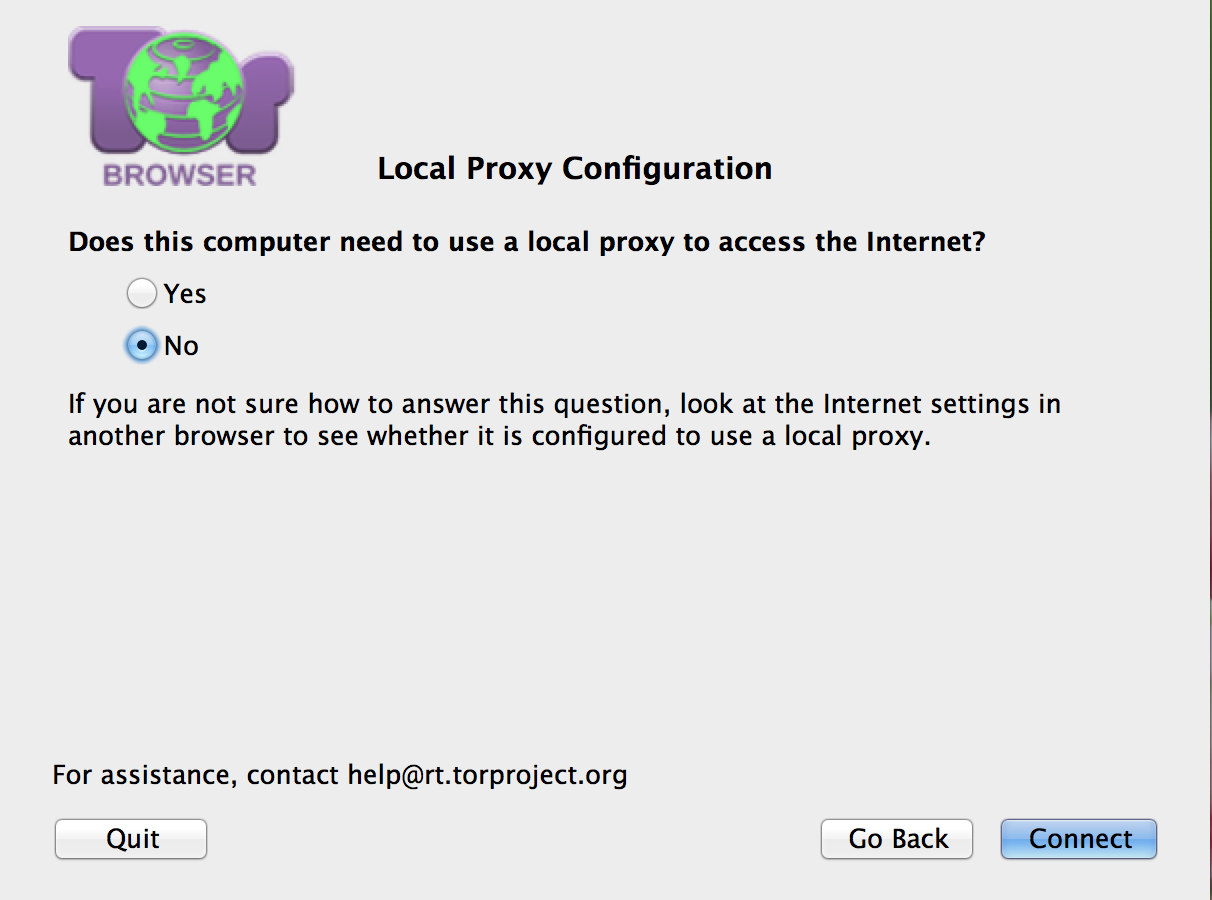
\includegraphics[width=0.5\textwidth]{window4.png}
    \caption{Window 4: This is the window shown after a user has deemed that a bridge
    is not required for the connection, or when the bridge configuration settings have been 
    chosen. Note that the default answer to if the user requires a proxy is ``No.'' Additionally,
    there is text to guide the users on how to answer this question. The user 
    can navigate to the previous window by clicking ``Go Back,'' and continue configuration 
    by clicking  ``Continue.''}
\end{figure}

\begin{figure}[h]
\label{fig:window5}
  \centering
    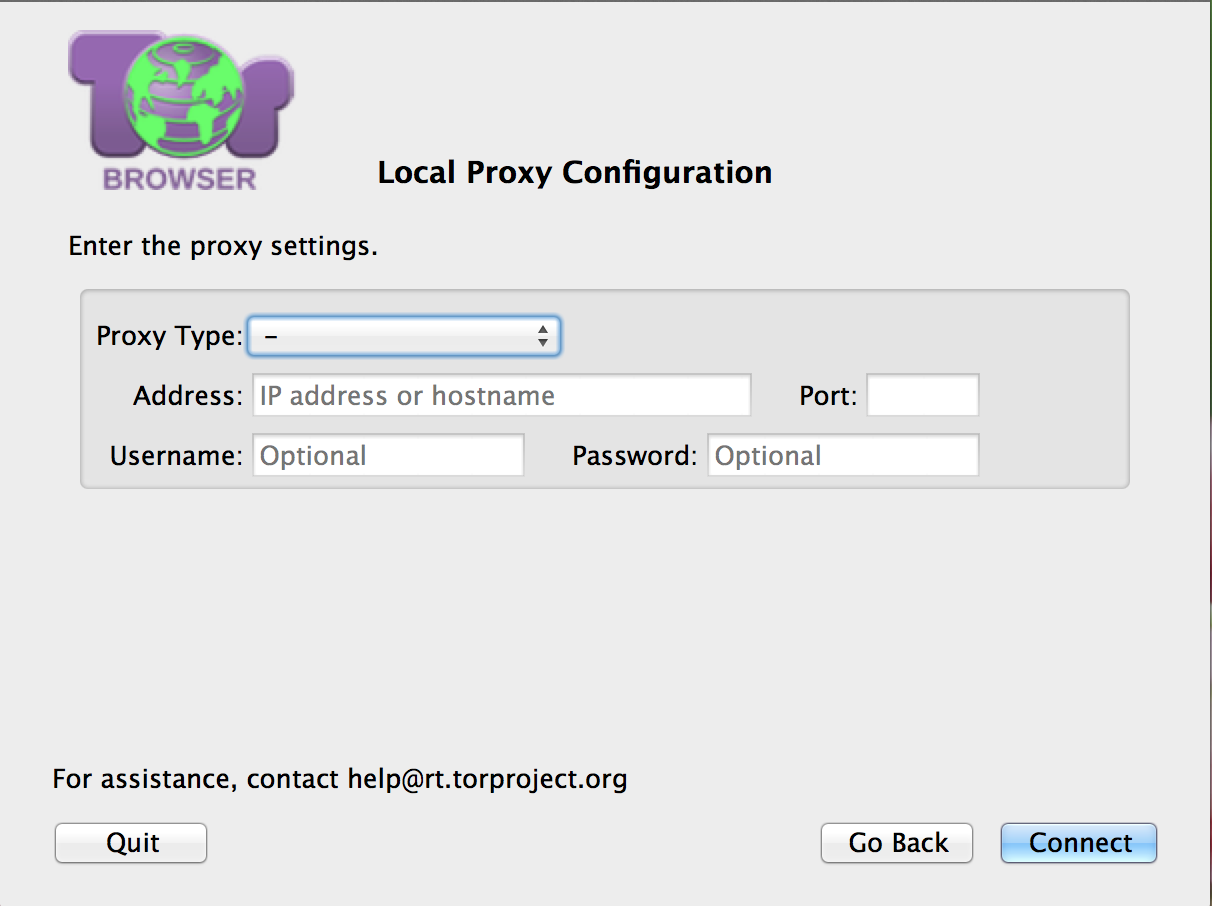
\includegraphics[width=0.5\textwidth]{window5.png}
    \caption{Window 5: This is the window shown when a user answers that a proxy is 
    required for the connection. Note that there are no default values in the answers, 
    where there were for bridges. Additionally, since this is the last window in the configuration
    interface, the options to navigate to other windows are to simply ``go back,'' or to 
    connect to the Tor Network.}
\end{figure}
\end{document}
